\documentclass[tikz, border=10px]{standalone}
\usetikzlibrary{automata, positioning, arrows.meta, calc}

\begin{document}
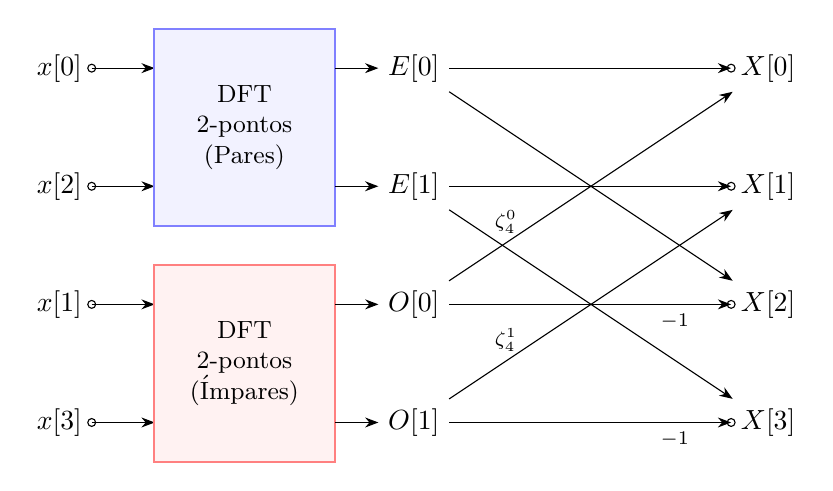
\begin{tikzpicture}[>=Stealth, node distance=1.5cm]

  % --- CONFIGURAÇÕES GERAIS ---
  % Espaçamento vertical entre linhas
  \def\dy{1.5} 
  
  % --- ENTRADA (Bit-Reversal) ---
  % Pares (Evens)
  \node (x0) at (0, 0) {$x[0]$};
  \node (x2) at (0, -\dy) {$x[2]$};
  % Ímpares (Odds)
  \node (x1) at (0, -2*\dy) {$x[1]$};
  \node (x3) at (0, -3*\dy) {$x[3]$};

  % Pequenos círculos nos inputs
  \foreach \n/\i in {x0/0, x2/1, x1/2, x3/3} {
    \draw [fill=white] (\n.east) circle (0.05);
    \draw [->] (\n.east) -- ++(0.8, 0);
  }

  % --- BLOCOS RECURSIVOS (N/2 DFTs) ---
  % Bloco Superior (DFT de 2 pontos para os Pares)
  \draw[fill=blue!5, draw=blue!50, thick] (1.2, 0.5) rectangle (3.5, -\dy - 0.5);
  \node at (2.35, -0.5*\dy) [align=center, font=\small] {DFT\\2-pontos\\(Pares)};

  % Bloco Inferior (DFT de 2 pontos para os Ímpares)
  \draw[fill=red!5, draw=red!50, thick] (1.2, -2*\dy + 0.5) rectangle (3.5, -3*\dy - 0.5);
  \node at (2.35, -2.5*\dy) [align=center, font=\small] {DFT\\2-pontos\\(Ímpares)};

  % --- SAÍDAS INTERMEDIÁRIAS (E e O) ---
  % Saídas Pares (E)
  \node (E0) at (4.5, 0) {$E[0]$};
  \node (E1) at (4.5, -\dy) {$E[1]$};
  
  % Saídas Ímpares (O)
  \node (O0) at (4.5, -2*\dy) {$O[0]$};
  \node (O1) at (4.5, -3*\dy) {$O[1]$};

  % Conectando blocos aos nós intermediários
  \draw [->] (3.5, 0) -- (E0);
  \draw [->] (3.5, -\dy) -- (E1);
  \draw [->] (3.5, -2*\dy) -- (O0);
  \draw [->] (3.5, -3*\dy) -- (O1);

  % --- ESTÁGIO DE COMBINAÇÃO (BUTTERFLY) ---
  
  % Nós de Saída Final (X)
  \node (X0) at (9, 0) {$X[0]$};
  \node (X1) at (9, -\dy) {$X[1]$};
  \node (X2) at (9, -2*\dy) {$X[2]$};
  \node (X3) at (9, -3*\dy) {$X[3]$};

  % Círculos nas saídas
  \foreach \n in {X0, X1, X2, X3} {
    \draw [fill=white] (\n.west) circle (0.05);
  }

  % --- CONEXÕES DO DIAGRAMA BORBOLETA ---
  
  % Linhas retas (Pares vão direto)
  \draw [->] (E0) -- (X0); % E[0] -> X[0]
  \draw [->] (E1) -- (X1); % E[1] -> X[1]
  \draw [->] (E0) -- (X2); % E[0] -> X[2]
  \draw [->] (E1) -- (X3); % E[1] -> X[3]

  % Linhas cruzadas (Ímpares com Twiddle Factors)
  % O[0] caminhos
  \draw [->] (O0) -- node[above, pos=0.2, font=\scriptsize] {$\zeta_4^0$} (X0); % O[0] -> X[0]
  \draw [->] (O0) -- node[below, pos=0.8, font=\scriptsize] {$-1$} (X2);   % O[0] -> X[2] (Subtração)

  % O[1] caminhos
  \draw [->] (O1) -- node[above, pos=0.2, font=\scriptsize] {$\zeta_4^1$} (X1); % O[1] -> X[1]
  \draw [->] (O1) -- node[below, pos=0.8, font=\scriptsize] {$-1$} (X3);   % O[1] -> X[3] (Subtração)

  % Detalhes visuais nos cruzamentos (Pequenos círculos de soma)
  % Não estritamente necessário, mas ajuda na leitura
  \foreach \target in {X0, X1, X2, X3} {
     %\node[circle, draw, inner sep=1pt, fill=white] at ($(\target.west) + (-0.2,0)$) {\tiny +};
  }

\end{tikzpicture}
\end{document}